\documentclass[12pt]{article}
\usepackage{helvet}
\usepackage{graphicx}
\usepackage{geometry}
\geometry{
    a4paper,
    top = 2cm,
    left = 2cm,
    right = 2cm,
    bottom = 3cm
}
\usepackage[utf8]{inputenc}
\usepackage[spanish,mexico]{babel} % Renombra en automático los elementos a español
\addto\captionsspanish{
  \renewcommand{\figurename}{Imagen}
  \renewcommand{\tablename}{Tabla}
}
\usepackage{float}  % Etiqueta 'H' (mayus) en figuras (imágenes)
\usepackage{array}  % Padding en tablas
\usepackage{tabularx}
\usepackage{url}    % Etiqueta url en .bib
\usepackage{booktabs}   % Manejo de caudros (tablas)
\usepackage[T1]{fontenc}    % Codificación de fuentes
\usepackage[autostyle, spanish=mexican]{csquotes}       % Paquete para comillas tipográficas
\usepackage{comment}    % Comentar bloques de líneas mediante begin-end
\usepackage{multicol}   % Para poner contenido a doble columna
\usepackage{enumitem}   % Para utilizar [noitemsep, topsep=0pt] en itemize
\usepackage{amsmath}
\usepackage{mathabx} % Para testar en math mode
\usepackage{comment}
\usepackage{longtable}
\usepackage[hidelinks]{hyperref}
\usepackage{caption}
\usepackage[
  backend=biber,
  style=apa,
  sorting=nyt
]{biblatex}
\DeclareLanguageMapping{spanish}{spanish-apa}
\renewcommand{\familydefault}{\sfdefault}
\newenvironment{localsubgroup}
  {$\left\{\tabular{l}}
  {\endtabular\right.$}


\addbibresource{bibliography/t03.bib}

\begin{comment}
Indicaciones del profesor:

a) Investigar:
- Las teclas de atajo más utilizadas en Windows
 Ej. Abrir explorador de archivos
- ¿Teclas de acceso rápido en GNU/Linux y mencionar el sistema utilizado?
 Ej. Abrir la terminal
 Ej. ¿Cómo hago una captura de pantalla en Linux?

b) Investigar:
- ¿Qué es el editor vi?
- ¿Cómo funciona el editor vi?
- Realiza un ejemplo con capturas de pantalla.

c) Investigar:
- 10 comandos para terminal en Linux
- 10 comandos para uso de CMD en Windows 10/11
- ¿Qué se entiende por ruta absoluta y ruta relativa?

Un máximo de 25 hojas.

Rango normativo: 18 a 25 páginas (objetivo ajustado a ~22-24 páginas para respetar el límite de 25 hojas del profesor).

Índice aprobado:
1. Fundamentos de intercepción de eventos y atajos de teclado [1.5 págs.]
   1.1. Captura de eventos de entrada y arquitectura del subsistema
   1.2. Mecanismos de registro global y atajos de aplicación
2. Atajos de teclado en Microsoft Windows [2.0 págs.]
   2.1. Procesamiento de mensajes y API en Win32k
   2.2. Catálogo técnico de combinaciones esenciales
3. Atajos de teclado en entornos GNU/Linux [2.0 págs.]
   3.1. Servidores gráficos: X11 y compositores Wayland
   3.2. Catálogo de atajos en entorno GNOME sobre Wayland
   3.3. Mecanismos y herramientas de captura de pantalla
4. Arquitectura y modelo modal del editor Vi [1.5 págs.]
   4.1. Evolución histórica: de ex a POSIX.1 y Vim
   4.2. Máquina de estados finitos y modos de ejecución
5. Operativa, gramática de comandos y flujo en Vi [2.0 págs.]
   5.1. Composición sintáctica: operadores, conteos y movimientos
   5.2. Manipulación de búferes, registros y sustitución
6. Demostración práctica de edición en Vim [2.5 págs.]
   6.1. Inicialización de sesión y modo Normal
   6.2. Captura y modificación en modo Inserción
   6.3. Operaciones estructurales en modo Normal
   6.4. Selección por bloques en modo Visual
   6.5. Comandos de sustitución y persistencia en modo Ex
7. Estructura de directorios: rutas absolutas y relativas [2.0 págs.]
   7.1. Jerarquía del sistema de archivos y directorio de trabajo
   7.2. Definición formal de ruta absoluta y ruta relativa
   7.3. Mecanismos de resolución en núcleos POSIX y Windows NT
8. Comandos de terminal en sistemas GNU/Linux [2.5 págs.]
   8.1. Arquitectura del shell y ejecución de utilidades
   8.2. Catálogo de diez comandos fundamentales
9. Comandos del intérprete CMD en Windows [2.5 págs.]
   9.1. Arquitectura de cmd.exe y llamadas al sistema
   9.2. Catálogo de diez comandos fundamentales
10. Análisis comparativo de interfaces y direccionamiento [1.5 págs.]
    10.1. Comparativa entre entornos de línea de comandos
    10.2. Diferencias operativas en la gestión de rutas
11. Conclusiones personales [2.0 págs.]
Referencias [1.0 - 1.5 págs.]
\end{comment}

\begin{document}
\pagenumbering{roman}

\begin{titlepage}
  \thispagestyle{empty}
  \newgeometry{left = 1cm, right = 1cm, top = 1cm, bottom = 2cm}

  \noindent
  \begin{minipage}[c]{3.5cm}
    
\includegraphics[width=3.5cm]{media/titlepage/Escudo-UNAM.pdf}
  \end{minipage}\hfill
  \begin{minipage}[c][3.5cm][c]{\dimexpr\textwidth-7cm\relax}
    \centering
    {\large\textbf{Universidad Nacional Autónoma de México}\\[0.6em] 
    \Large\textbf{Facultad de Ingeniería}\\[0.6em]
    \large Sistemas Operativos}
  \end{minipage}\hfill
  \begin{minipage}[c]{3.5cm}
    \raggedleft
    
\includegraphics[width=3.5cm]{media/titlepage/FI.png}
  \end{minipage}
\centering\huge
  \vfill
    Grupo 1 \\
    Ing. Angel Isidro Mercado
  \vfill
    \textbf{Tarea 3. Atajos, Vi y comandos}
  \vfill\large
    320304435 - Cabrera Rojas Oscar
  \vfill

  \noindent\footnotesize \hfill Ciudad Universitaria, CDMX a 22 de septiembre del 2026
\end{titlepage}
\restoregeometry

\tableofcontents

\newpage
\pagenumbering{arabic}
\setcounter{page}{1}

\section{Fundamentos de intercepción de eventos y atajos de teclado}
\label{sec:fundamentosIntercepcionEventos}

El teclado constituye el dispositivo primario de interacción en los sistemas operativos modernos. Desde la perspectiva del usuario, un atajo de teclado representa una pulsación simultánea o secuencial destinada a ejecutar una función expedita. Sin embargo, a nivel de arquitectura del sistema operativo, esta acción desencadena una cadena asíncrona de eventos que enlaza el hardware con el espacio de usuario \parencite[\S 13.2, p.\ 450]{silberschatz2006fundamentos}.

\subsection{Captura de eventos de entrada y arquitectura del subsistema}
\label{subsec:capturaEventosEntrada}

La pulsación física en la matriz del teclado induce al microcontrolador integrado a sintetizar un código de escaneo binario (\textit{scancode}), diferenciando entre el código de activación (\textit{make code}) y el de liberación (\textit{break code}). Esta asimetría permite al sistema detectar teclas modificadoras sostenidas (Shift, Control, Alt) \parencite[\S 7.8, p.\ 399]{carretero2001sistemas}. La transferencia hacia la placa base se canaliza mediante interfaces USB HID o el controlador 8042, disparando una interrupción física (IRQ) en el controlador APIC.

Para maximizar el rendimiento, el núcleo divide la atención en dos fases: la mitad superior (\textit{top half} o ISR mínima) almacena el scancode en una cola circular de memoria, mientras que la mitad inferior (\textit{bottom half}, como DPC en Windows o \textit{tasklets} en Linux) traduce el código a una clave virtual universal \parencite[\S 1.4, p.\ 40]{stallings2018operating}. En GNU/Linux, el subsistema \texttt{evdev} expone estructuras \texttt{input\_event} a través de \texttt{/dev/input/event*} procesadas por \texttt{libinput}; en Windows NT, el controlador \texttt{kbdclass.sys} entrega los paquetes al hilo de entrada cruda (\textit{raw input thread}, RIT) en \texttt{win32k.sys} \parencite{microsoftRegisterHotKey}.

\subsection{Mecanismos de registro global y atajos de aplicación}
\label{subsec:mecanismosRegistroGlobal}

Al recibir el evento normalizado, el subsistema gráfico determina si se trata de un atajo global del sistema o un acelerador local de aplicación. Los atajos globales (\textit{global hotkeys}) actúan independientemente de la ventana enfocada. En Microsoft Windows, se registran mediante la API \texttt{RegisterHotKey}, haciendo que el hilo RIT intercepte la combinación y despache un mensaje \texttt{WM\_HOTKEY} prioritario al hilo correspondiente \parencite{microsoftRegisterHotKey}. En GNU/Linux bajo Wayland, el compositor gráfico asume el control exclusivo del teclado para prevenir el espionaje (\textit{keylogging}) propio de la arquitectura histórica X11 (\texttt{XGrabKey}), canalizando atajos de terceros mediante el portal de escritorio XDG \texttt{org.freedesktop.portal.GlobalShortcuts} sobre D-Bus con autorización explícita del usuario \parencite{freedesktopGlobalShortcuts}.

Si una combinación no coincide con un registro global, los eventos se despachan al proceso en primer plano, donde las tablas de aceleradores (\texttt{TranslateAccelerator} en Win32) o controladores de \textit{toolkits} (GTK, Qt) mapean las pulsaciones a comandos internos. La Tabla~\ref{tab:procesamientoAtajosSo} sintetiza este flujo multidimensional en el sistema operativo.

\begin{table}[htbp]
\centering
\footnotesize
\renewcommand{\arraystretch}{1.1}
\renewcommand{\tabularxcolumn}[1]{m{#1}}
\setlength{\emergencystretch}{1.5em}
\caption{Niveles de procesamiento e intercepción de atajos en el sistema operativo.}
\label{tab:procesamientoAtajosSo}
\begin{tabularx}{\textwidth}{>{\centering\arraybackslash}m{2.8cm} X X}
\toprule
\textbf{Nivel} & \textbf{Componentes y flujo de señales} & \textbf{Resolución y alcance del atajo} \\
\midrule
\textbf{Hardware / Firmware} & Matriz física, microcontrolador y controlador USB HID / 8042. & Genera \textit{scancodes} crudos y dispara interrupciones físicas (IRQ) hacia la CPU. \\
\addlinespace
\textbf{Núcleo del SO} & Rutina ISR, mitades inferiores (DPC / \textit{tasklets}), subsistema \texttt{evdev} / \texttt{kbdclass.sys}. & Decodifica scancodes, procesa teclas modificadoras y sintetiza códigos virtuales normalizados. \\
\addlinespace
\textbf{Servidor / Compositor} & Subsistema Win32k (hilo RIT) o compositor Wayland / servidor X11. & Evalúa capturas globales (\texttt{RegisterHotKey}, portales XDG). Desvía atajos del entorno de escritorio. \\
\addlinespace
\textbf{Espacio de usuario} & Bucle de mensajes del proceso enfocado y tablas de aceleradores (GTK, Qt, Win32). & Interpreta eventos dirigidos a la ventana activa (ej. \texttt{Ctrl+S}), mapeándolos a funciones internas. \\
\bottomrule
\end{tabularx}
\end{table}

\section{Atajos de teclado en Microsoft Windows}
\label{sec:atajosTecladoWindows}

En el sistema operativo Microsoft Windows, los atajos de teclado constituyen una parte integral de la experiencia de usuario y de la administración del sistema. Su funcionamiento se apoya en una arquitectura híbrida donde los controladores del núcleo, el subsistema gráfico de ventanas y el intérprete de interfaz cooperan estrechamente para traducir combinaciones de teclas en acciones ejecutivas inmediatas. Esta sección examina la infraestructura interna que procesa estos eventos en el núcleo de Windows y desglosa las combinaciones más utilizadas en las versiones Windows 10 y Windows 11.

\subsection{Procesamiento de mensajes y API en Win32k}
\label{subsec:procesamientoWin32k}

La arquitectura de interfaz de Windows aloja sus subsistemas críticos (USER y GDI) en espacio de núcleo dentro de \texttt{win32k.sys} y \texttt{win32kbase.sys} para suprimir la sobrecarga por cambios de contexto entre modos de ejecución \parencite[\S 21.4, p.\ 1043]{deitel2004operating}. El flujo de teclado es administrado por el hilo de entrada cruda (RIT), que extrae paquetes de \texttt{kbdclass.sys} y gestiona los estados de teclas modificadoras \parencite{microsoftKeyboardInput}.

Al recibir una pulsación, el RIT aplica una estricta jerarquía de intercepción: primero evalúa la secuencia de atención segura (SAS, \texttt{Ctrl + Alt + Del}), desviándola exclusivamente al proceso \texttt{winlogon.exe} en el escritorio seguro para impedir la captura maliciosa de credenciales; en segundo término, verifica las combinaciones globales dadas de alta con \texttt{RegisterHotKey}, despachando un mensaje \texttt{WM\_HOTKEY} prioritario al hilo registrado; y finalmente, si no hay intercepción, deposita los eventos ordinarios (\texttt{WM\_KEYDOWN}, \texttt{WM\_CHAR}) en la cola de la ventana con foco de entrada \parencite{microsoftRegisterHotKey}.

\subsection{Catálogo técnico de combinaciones esenciales}
\label{subsec:catalogoAtajosWindows}

Las combinaciones de teclas más utilizadas en Windows 10 y Windows 11 se articulan en torno a la administración del almacenamiento, el control de procesos, la composición espacial de ventanas y la captura gráfica \parencite{microsoftShortcutsWindows}.

En la exploración y administración de archivos, la combinación más representativa es \texttt{Win + E}, que invoca una nueva instancia de \texttt{explorer.exe} en la vista de acceso rápido o en la raíz local. Dentro del explorador, \texttt{Alt + Flecha Arriba} asciende en el árbol jerárquico, \texttt{Alt + Flecha Izquierda} conmuta al directorio previo en el historial, \texttt{F2} edita el nombre del nodo seleccionado y \texttt{Ctrl + Shift + N} crea inmediatamente una nueva carpeta en el CWD. Para el control del sistema, \texttt{Ctrl + Shift + Esc} invoca directamente el Administrador de Tareas (\texttt{taskmgr.exe}) con prioridad ejecutiva elevada, permitiendo diagnosticar y forzar la terminación de procesos aun si el shell gráfico está bloqueado. Asimismo, \texttt{Win + R} abre el cuadro de ejecución (\texttt{RunFileDlg} en \texttt{shell32.dll}) para binarios y consolas administrativas resueltas mediante \texttt{PATH}, \texttt{Win + X} despliega el Menú de Enlace Rápido (\textit{Power User Menu}) y \texttt{Win + I} abre la Configuración mediante el protocolo \texttt{ms-settings:}.

En la gestión de ventanas y superficies, el Administrador de Ventanas del Escritorio (DWM) coordina la manipulación espacial. El atajo \texttt{Alt + Tab} conmuta entre aplicaciones activas alterando su orden de profundidad (\textit{z-order}), mientras que \texttt{Win + Tab} activa la Vista de Tareas. La creación de nuevos escritorios virtuales se realiza con \texttt{Win + Ctrl + D}, la navegación horizontal entre ellos con \texttt{Win + Ctrl + Flecha Izquierda / Derecha}, y su desasignación con \texttt{Win + Ctrl + F4}. Para la organización en mosaico, \texttt{Win + Flechas de dirección} calcula el rectángulo delimitador mediante la API \texttt{SetWindowPos} (\textit{Snap Assist}), \texttt{Win + D} minimiza o restaura en bloque las ventanas visibles, y \texttt{Win + L} invoca \texttt{LockWorkStation} en \texttt{user32.dll} transfiriendo la pantalla al entorno seguro de autenticación.

Finalmente, en el dominio de captura gráfica y portapapeles, \texttt{Win + Shift + S} invoca la herramienta de recortes (\texttt{SnippingTool.exe}), congelando el fotograma del DWM y depositando la región seleccionada en el portapapeles en formatos DIB y PNG \parencite{microsoftShortcutsWindows}. Esta función se complementa con \texttt{Win + V}, que abre el historial del portapapeles administrado por el servicio \textit{Clipboard Broker Service}. Para capturas directas, \texttt{Impr Pant} copia la pantalla completa y \texttt{Alt + Impr Pant} restringe la muestra a la geometría de la ventana con foco.

La Tabla~\ref{tab:catalogoAtajosWindows} sintetiza las principales combinaciones de teclado en Microsoft Windows, vinculando cada atajo con el componente del sistema operativo que lo procesa y su impacto técnico en la ejecución del entorno.

\begin{table}[htbp]
\centering
\footnotesize
\renewcommand{\arraystretch}{1.08}
\renewcommand{\tabularxcolumn}[1]{m{#1}}
\setlength{\emergencystretch}{1.5em}
\caption{Catálogo técnico de atajos de teclado esenciales en Microsoft Windows.}
\label{tab:catalogoAtajosWindows}
\begin{tabularx}{\textwidth}{>{\centering\arraybackslash}m{2.8cm} X X}
\toprule
\textbf{Atajo de teclado} & \textbf{Componente / Proceso} & \textbf{Mecanismo y acción técnica en el SO} \\
\midrule
\texttt{Win + E} & Shell (\texttt{explorer.exe}) & Instancia una nueva ventana del Explorador de archivos sobre el espacio de nombres virtual del sistema. \\
\addlinespace
\texttt{Ctrl + Shift + Esc} & Núcleo / \texttt{taskmgr.exe} & Invocación prioritaria del Administrador de Tareas para monitoreo de hilos y terminación de procesos. \\
\addlinespace
\texttt{Win + R} & \texttt{shell32.dll} (\texttt{RunFileDlg}) & Abre el cuadro de ejecución que resuelve rutas de binarios y consolas administrativas en el \texttt{PATH}. \\
\addlinespace
\texttt{Win + X} & Menú del sistema (\textit{Quick Link}) & Despliega accesos directos administrativos predefinidos (Terminal elevada, Administrador de discos). \\
\addlinespace
\texttt{Win + L} & \texttt{user32.dll} (\texttt{LockWorkStation}) & Bloquea la sesión de usuario y conmuta la pantalla al escritorio seguro gestionado por \texttt{winlogon.exe}. \\
\addlinespace
\texttt{Win + D} & Gestor de ventanas / DWM & Conmuta el estado de visibilidad del escritorio, minimizando o restaurando todas las ventanas activas. \\
\addlinespace
\texttt{Alt + Tab} & Compositor DWM & Alterna el foco del teclado y reordena la pila de ventanas según su jerarquía de profundidad (\textit{z-order}). \\
\addlinespace
\texttt{Win + Tab} & Vista de tareas / DWM & Presenta la vista panorámica de ventanas y paneles de administración de escritorios virtuales. \\
\addlinespace
\texttt{Win + Ctrl + D} & Gestor de sesiones / DWM & Crea e inicializa dinámicamente una nueva superficie de escritorio virtual en la sesión interactiva. \\
\addlinespace
\texttt{Win + Flechas} & API Win32 (\texttt{SetWindowPos}) & Asistente de anclaje (\textit{Snap Assist}): redimensiona y ajusta la ventana en mitades o cuadrantes. \\
\addlinespace
\texttt{Win + Shift + S} & Herramienta de recortes & Congela el fotograma del DWM y exporta la región seleccionada al portapapeles en formato DIB/PNG. \\
\addlinespace
\texttt{Win + V} & \textit{Clipboard Broker Service} & Despliega el historial persistente de elementos almacenados en el búfer múltiple del portapapeles. \\
\bottomrule
\end{tabularx}
\end{table}

\section{Atajos de teclado en entornos GNU/Linux}
\label{sec:atajosTecladoLinux}

En los sistemas operativos basados en el núcleo Linux, la arquitectura gráfica y el procesamiento de eventos de teclado se fundamentan en una separación modular entre el kernel, el servidor o compositor gráfico y el entorno de escritorio. Como sistema de referencia formal para el presente análisis, se toma una distribución GNU/Linux moderna ejecutando el entorno GNOME (versión 40 en adelante) sobre el compositor Mutter bajo el protocolo Wayland, contrastándolo con la arquitectura clásica de X11.

\subsection{Servidores gráficos: X11 y compositores Wayland}
\label{subsec:servidoresGraficosLinux}

En la arquitectura histórica de X11, el servidor centralizado Xorg capturaba atajos globales mediante la función \texttt{XGrabKey}, desviando eventos al cliente solicitante. No obstante, la ausencia de aislamiento permitía que cualquier proceso leyera arbitrariamente el flujo global del teclado (\textit{keylogging}).

Bajo Wayland, el servidor gráfico, el gestor de ventanas y el compositor se unifican en un único proceso (Mutter en GNOME) que interactúa directamente con el núcleo vía KMS/DRM y \texttt{libinput}. Wayland impone un aislamiento estricto de superficies: cada aplicación solo recibe eventos cuando posee el foco activo. Los atajos globales del sistema son evaluados y consumidos internamente por el compositor, mientras que las aplicaciones enjauladas (Flatpak) deben solicitar atajos mediante el portal XDG \texttt{org.freedesktop.portal.GlobalShortcuts} sobre D-Bus, requiriendo autorización explícita del usuario \parencite{freedesktopGlobalShortcuts}.

\subsection{Catálogo de atajos en entorno GNOME sobre Wayland}
\label{subsec:catalogoAtajosGnome}

El entorno de escritorio GNOME provee un catálogo estandarizado de atajos procesados por \texttt{gnome-settings-daemon} y el compositor Mutter \parencite{gnomeShellShortcuts}. La invocación del intérprete de comandos mediante \texttt{Ctrl + Alt + T} despacha la terminal predeterminada instanciando un proceso hijo vinculado a un pseudoterminal (\textit{pty}) mediante las llamadas \texttt{fork()} y \texttt{execve()}. Para el lanzamiento de aplicaciones y supervisión, la tecla \texttt{Super} activa la Vista General de Actividades, exponiendo un mosaico de ventanas junto a la gestión de espacios de trabajo dinámicos, navegables horizontalmente con \texttt{Super + Re Pág / Av Pág}, mientras que \texttt{Alt + F2} abre el cuadro de ejecución directa.

La manipulación espacial de superficies se coordina mediante atajos del compositor: \texttt{Alt + Tab} conmuta entre aplicaciones reordenando el plano visual, \texttt{Alt + `} alterna entre ventanas de una misma aplicación (\textit{window cycling}), y \texttt{Super + Flechas} ajusta ventanas en mitades simétricas o maximización. Para seguridad y control de sesión, \texttt{Super + L} transfiere el control a GDM mediante D-Bus bloqueando la pantalla, y \texttt{Ctrl + Alt + Supr} despliega el diálogo de apagado. En el nivel más bajo del núcleo, las combinaciones de emergencia \texttt{Ctrl + Alt + F1--F6} conmutan fuera del servidor gráfico hacia consolas virtuales de texto puro (TTY) administradas por \texttt{systemd-vconsole-setup} \parencite[\S 7.8, p.\ 399]{carretero2001sistemas}.

\subsection{Mecanismos y herramientas de captura de pantalla}
\label{subsec:mecanismosCapturaPantalla}

La captura de pantalla en GNU/Linux bajo compositores modernos constituye un caso ejemplar de interacción entre atajos de teclado y mecanismos de seguridad del sistema operativo. Debido a que el protocolo Wayland prohíbe que cualquier cliente de usuario lea directamente los búferes de fotogramas del servidor, la captura debe ser efectuada directamente por el compositor o delegada mediante protocolos seguros.

En el entorno GNOME (a partir de la versión 42), la pulsación de \textbf{\texttt{PrintScreen}} (o \texttt{Impr Pant}) despliega una interfaz interactiva superpuesta (\textit{screenshot overlay}) integrada en Mutter y GNOME Shell \parencite{gnomeShellShortcuts}. Esta herramienta congela el fotograma y ofrece tres modalidades de selección: pantalla completa (abarca todos los monitores), ventana específica (delimita la geometría activa) o selección de área rectangular por coordenadas. Permite además alternar hacia la grabación de vídeo (\textit{screencast}). Al confirmarse, el compositor exporta la imagen a PNG en \texttt{\textasciitilde/Imágenes/Capturas de pantalla/} y copia los píxeles al portapapeles. Para capturas directas sin menú emergente, \texttt{Shift + PrintScreen} captura la pantalla completa, \texttt{Alt + PrintScreen} captura la ventana enfocada, y \texttt{Shift + Ctrl + Alt + R} activa el \textit{screencast} en tiempo real.

En aplicaciones enjauladas (Flatpak) o herramientas externas, la operación se canaliza a través del portal de escritorio XDG mediante \nolinkurl{org.freedesktop.portal.Screenshot} sobre D-Bus \parencite{freedesktopScreenshotPortal}. El compositor Mutter solicita confirmación al usuario y deposita el archivo en un sistema de archivos virtual seguro (\texttt{/run/user/\$UID/doc/}), impidiendo capturas silenciosas no autorizadas. En entornos de línea de comandos, destacan utilidades como \texttt{gnome-screenshot}, \texttt{grim} (vía el protocolo Wayland \texttt{wlr-screencopy-unstable-v1}) y \texttt{slurp} para la selección interactiva de geometrías.

La Tabla~\ref{tab:catalogoAtajosGnome} resume las combinaciones de teclas más representativas en GNU/Linux bajo GNOME y Wayland, su componente de procesamiento y su repercusión técnica en el sistema operativo.

\begin{table}[htbp]
\centering
\footnotesize
\renewcommand{\arraystretch}{1.08}
\renewcommand{\tabularxcolumn}[1]{m{#1}}
\setlength{\emergencystretch}{1.5em}
\caption{Catálogo técnico de atajos esenciales en GNU/Linux (GNOME sobre Wayland).}
\label{tab:catalogoAtajosGnome}
\begin{tabularx}{\textwidth}{>{\centering\arraybackslash}m{2.8cm} X X}
\toprule
\textbf{Atajo de teclado} & \textbf{Componente / Servicio} & \textbf{Mecanismo y acción técnica en el SO} \\
\midrule
\texttt{Ctrl + Alt + T} & \texttt{gnome-settings-daemon} & Invoca la terminal predeterminada (\texttt{fork} y \texttt{execve} asociados a un nuevo \textit{pty}). \\
\addlinespace
\texttt{PrintScreen} & GNOME Shell / Mutter & Despliega la interfaz interactiva de captura (pantalla, ventana o área) y \textit{screencast}. \\
\addlinespace
\texttt{Shift + PrintScreen} & Compositor Mutter & Captura directa de la pantalla completa y almacenamiento atómico en formato PNG. \\
\addlinespace
\texttt{Alt + PrintScreen} & Compositor Mutter & Captura exclusiva de la superficie geométrica de la ventana con foco activo. \\
\addlinespace
\texttt{Super} & GNOME Shell & Conmuta a la Vista General de Actividades, exponiendo mosaico de ventanas y escritorios. \\
\addlinespace
\texttt{Super + Re Pág / Av Pág} & Gestor de espacios dinámicos & Navegación horizontal entre escritorios virtuales asignados dinámicamente en memoria. \\
\addlinespace
\texttt{Alt + Tab} & Compositor Mutter & Conmuta el foco de entrada entre aplicaciones activas alterando la jerarquía visual. \\
\addlinespace
\texttt{Alt + `} & GNOME Shell & Conmutación interna de ventanas (\textit{window cycling}) entre instancias de una misma aplicación. \\
\addlinespace
\texttt{Super + Flechas} & Compositor Mutter & Ajuste geométrico de superficies: maximización vertical o división en mitades laterales. \\
\addlinespace
\texttt{Super + L} & GDM (\texttt{org.gnome.ScreenSaver}) & Bloquea la sesión y transfiere la salida gráfica al protector de pantalla autenticado. \\
\addlinespace
\texttt{Ctrl + Alt + F1--F6} & Núcleo Linux / TTY & Conmuta fuera del servidor gráfico hacia consolas virtuales de texto puro del sistema. \\
\bottomrule
\end{tabularx}
\end{table}

\section{Arquitectura y modelo modal del editor Vi}
\label{sec:arquitecturaModeloVi}

En los sistemas operativos tipo UNIX y las distribuciones GNU/Linux, el editor de texto es una herramienta crítica para la administración remota mediante SSH y consolas de rescate. En este contexto, \texttt{vi} y su versión extendida Vim (\textit{Vi IMproved}) representan el estándar de edición modal interactiva en interfaces textuales (\textit{text user interface}, TUI).

\subsection{Evolución histórica: de ex a POSIX.1 y Vim}
\label{subsec:evolucionHistoricaVi}

La génesis de \texttt{vi} data de 1976, cuando Bill Joy diseñó el editor extendido \texttt{ex} para BSD UNIX a partir del clásico editor de líneas \texttt{ed}, introduciendo un modo visual de pantalla completa (\texttt{vi}). El diseño ergonómico estuvo determinado por la terminal Lear Siegler ADM-3A, cuya carencia de teclas de cursor motivó el uso de las teclas alfanuméricas \texttt{h}, \texttt{j}, \texttt{k} y \texttt{l} para el desplazamiento bidimensional, y cuya tecla \textit{home} originó la tilde (\texttt{\textasciitilde}) para el directorio del usuario.

En 1992, la norma IEEE Std 1003.2 (consolidada en POSIX.1, IEEE Std 1003.1) estandarizó a \texttt{vi} como la utilidad de pantalla obligatoria para sistemas compatibles con UNIX \parencite{ieee2018posixvi}. Posteriormente, Bram Moolenaar presentó en 1991 la primera versión de Vim, introduciendo resaltado sintáctico, árbol de deshacer multinivel, ventanas divididas y selección visual estructurada \parencite{oualline2001vim, moolenaar2024vim}.

\subsection{Máquina de estados finitos y modos de ejecución}
\label{subsec:maquinaEstadosVi}

A diferencia de los editores convencionales, Vi opera como una máquina de estados finitos (FSM) determinista, donde la semántica de cada tecla depende del modo activo: Normal (navegación y comandos sin modificadores continuos), Inserción (captura de texto en el búfer), Línea o Ex (directivas globales, entrada/salida y configuración), Visual (selección matricial de texto) y Reemplazo (sobrescritura secuencial). Para garantizar la tolerancia a fallos, el editor mantiene el texto en memoria RAM (búfer) y sincroniza transaccionalmente las páginas sucias en un archivo de intercambio oculto (\texttt{.swp}) en disco, habilitando la recuperación ante caídas del sistema (\texttt{vim -r}) y funcionando como cerrojo (\textit{lockfile}) ante accesos concurrentes \parencite{oualline2001vim}. La Tabla~\ref{tab:modosEjecucionVi} resume estos modos operativos y sus transiciones.

\begin{table}[htbp]
\centering
\footnotesize
\renewcommand{\arraystretch}{1.08}
\renewcommand{\tabularxcolumn}[1]{m{#1}}
\setlength{\emergencystretch}{1.5em}
\caption{Estados de la máquina modal en el editor Vi/Vim.}
\label{tab:modosEjecucionVi}
\begin{tabularx}{\textwidth}{>{\centering\arraybackslash}m{2.8cm} X X}
\toprule
\textbf{Modo} & \textbf{Activación y retorno} & \textbf{Semántica y función en el SO} \\
\midrule
\textbf{Normal} & Estado inicial; retorno con \texttt{<Esc>} o \texttt{Ctrl + [}. & Comandos de navegación y operadores léxicos en la fila central del teclado. \\
\addlinespace
\textbf{Inserción} & Operadores \texttt{i}, \texttt{I}, \texttt{a}, \texttt{A}, \texttt{o}, \texttt{O}, \texttt{s}. & Captura texto en el búfer en RAM; sincroniza periódicamente con el \texttt{.swp}. \\
\addlinespace
\textbf{Línea (Ex)} & Caracteres \texttt{:}, \texttt{/}, \texttt{?}; salida con \texttt{<Enter>}. & Interpreta órdenes en la última línea: I/O en disco (\texttt{:w}), salida y comandos de shell. \\
\addlinespace
\textbf{Visual} & Teclas \texttt{v} (carácter), \texttt{V} (línea), \texttt{Ctrl + v} (bloque). & Delimita regiones geométricas en pantalla para transformaciones atómicas. \\
\addlinespace
\textbf{Reemplazo} & Tecla \texttt{R}; retorno con \texttt{<Esc>}. & Sobrescribe los caracteres del búfer preservando la alineación visual circundante. \\
\bottomrule
\end{tabularx}
\end{table}

\section{Operativa, gramática de comandos y flujo en Vi}
\label{sec:operativaGramaticaVi}

El editor Vi formula cada instrucción siguiendo una gramática composicional formal basada en verbos y sustantivos:

\begin{equation}
\label{eq:gramaticaVi}
\text{Comando} = [\text{conteo}] + \text{operador} + [\text{conteo}] + \text{movimiento / objeto de texto}
\end{equation}

\subsection{Composición sintáctica: operadores, conteos y movimientos}
\label{subsec:composicionSintacticaVi}

Los operadores actúan como verbos ejecutivos en modo Normal: \texttt{d} (borrar/cortar), \texttt{c} (cambiar e ingresar a Inserción), \texttt{y} (copiar hacia registro), \texttt{>} / \texttt{<} (sangría) y \texttt{=} (reindentar). Al duplicarse (\texttt{dd}, \texttt{yy}), operan sobre la línea actual, y al prefijarse con un número (\texttt{3dd}), repiten la acción linealmente \parencite[\S 2, p.\ 35]{oualline2001vim}.

Los movimientos delimitan el alcance del operador o desplazan el cursor: caracteres y líneas (\texttt{hjkl}, \texttt{0}, \texttt{\textasciicircum}, \texttt{\$}), palabras (\texttt{w}, \texttt{b}, \texttt{e}), búsquedas en línea (\texttt{f}, \texttt{F}, \texttt{t}, \texttt{T}), estructuras sintácticas (\texttt{\{ \}}, \texttt{( )}, \texttt{\%} para pares) y saltos globales (\texttt{gg}, \texttt{G}). Asimismo, los objetos de texto (\textit{text objects}) permiten manipular entidades sintácticas internas (\texttt{iw}, \texttt{i\textquotedbl}, \texttt{i(}, \texttt{i\{}) o completas (\texttt{aw}, \texttt{a\textquotedbl}, \texttt{a\{}) desde cualquier punto en su interior \parencite{moolenaar2024vim}.

\subsection{Manipulación de búferes, registros y sustitución}
\label{subsec:manipulacionBuferesRegistros}

Vi desacopla la persistencia en disco de las estructuras de edición en memoria RAM (búferes), organizables en ventanas divididas (\texttt{:split}, \texttt{:vsplit}) y pestañas. Para transferencias de datos, implementa una matriz de registros desacoplada: el registro no nombrado (\texttt{\textquotedbl\textquotedbl}), 26 registros nombrados (\texttt{\textquotedbl a}--\texttt{\textquotedbl z}, admitiendo acumulación con mayúsculas), el registro de copia (\texttt{\textquotedbl 0}), el registro nulo (\texttt{\textquotedbl\_}) y los registros del portapapeles del sistema operativo (\texttt{\textquotedbl +} y \texttt{\textquotedbl *}) \parencite{moolenaar2024vim}.

La sustitución global se ejecuta en modo Ex con la directiva \texttt{s}:

\begin{equation}
\label{eq:sustitucionEx}
\text{:\hspace{0.2em}}[rango]\text{s}/patr\acute{o}n/reemplazo/[banderas]
\end{equation}

Donde \texttt{\%} abarca todo el archivo, \texttt{g} aplica el reemplazo a todas las ocurrencias por línea y \texttt{c} solicita confirmación interactiva. La Tabla~\ref{tab:gramaticaOperadoresVi} sintetiza esta gramática.

\begin{table}[htbp]
\centering
\footnotesize
\renewcommand{\arraystretch}{1.08}
\renewcommand{\tabularxcolumn}[1]{m{#1}}
\setlength{\emergencystretch}{1.5em}
\caption{Sintaxis de operadores, movimientos y registros en Vi/Vim.}
\label{tab:gramaticaOperadoresVi}
\begin{tabularx}{\textwidth}{>{\centering\arraybackslash}m{2.8cm} X X}
\toprule
\textbf{Categoría} & \textbf{Instrucciones representativas} & \textbf{Función y semántica operativa} \\
\midrule
\textbf{Operadores nucleares} & \texttt{d} (borrar), \texttt{c} (cambiar), \texttt{y} (copiar), \texttt{>} / \texttt{<} (sangría), \texttt{=} (reindentar). & Verbos ejecutivos; actúan sobre un movimiento o línea completa si se duplican (\texttt{dd}). \\
\addlinespace
\textbf{Movimientos} & \texttt{w}, \texttt{b}, \texttt{e} (palabra); \texttt{0}, \texttt{\textasciicircum}, \texttt{\$} (línea); \texttt{f}, \texttt{t} (búsqueda); \texttt{gg}, \texttt{G} (archivo). & Delimitan la extensión geométrica de la orden o trasladan el cursor en el búfer. \\
\addlinespace
\textbf{Objetos de texto} & \texttt{iw}, \texttt{aw} (palabra); \texttt{i\textquotedbl}, \texttt{a\textquotedbl} (comillas); \texttt{i(}, \texttt{i\{} (bloques de código). & Permiten manipular bloques sintácticos internos o con delimitadores de forma directa. \\
\addlinespace
\textbf{Registros de memoria} & \texttt{\textquotedbl\textquotedbl} (defecto), \texttt{\textquotedbl a--z} (nombrados), \texttt{\textquotedbl 0} (copia), \texttt{\textquotedbl +} (portapapeles SO), \texttt{\textquotedbl\_} (nulo). & Matriz de memoria persistente durante la sesión; soporta acumulación y portapapeles del SO. \\
\addlinespace
\textbf{Sustitución regex} & \texttt{:\%s/origen/destino/g}, \texttt{:\%s/patrón/reemplazo/gc}. & Reemplazo global con expresiones regulares y confirmación interactiva en modo Ex. \\
\bottomrule
\end{tabularx}
\end{table}

\section{Demostración práctica de edición en Vim}
\label{sec:demostracionPracticaVim}

Para consolidar los principios del modelo modal y la gramática formal, se desarrolla una sesión práctica de edición de código en C empleando Vim nativo en GNU/Linux. El ejercicio documenta el ciclo de vida del archivo: inicialización y modo Normal, captura en modo Inserción, transformaciones estructurales, manipulación matricial de columnas y persistencia en disco mediante el modo Ex.

\subsection{Inicialización de sesión y modo Normal}
\label{subsec:inicializacionModoNormal}

La sesión inicia ejecutando \texttt{vim ejemplo\_so.c}. El proceso adquiere descriptores para \texttt{stdin}, \texttt{stdout} y \texttt{stderr}, conmuta el controlador TTY a modo crudo (\textit{raw mode}) desactivando el eco local, e inicializa en disco el archivo de intercambio \texttt{.ejemplo\_so.c.swp} para tolerancia a fallos. Vim sitúa al usuario en modo Normal en la coordenada $(1,1)$, donde las tildes (\texttt{\textasciitilde}) indican líneas fuera del búfer de memoria y la línea de estado confirma la creación de un nuevo búfer vacío \parencite[\S 2, p.\ 28]{oualline2001vim}, como se ilustra en la Img.~\ref{fig:vimModoNormalInicio}.

\begin{figure}[htbp]
    \centering
    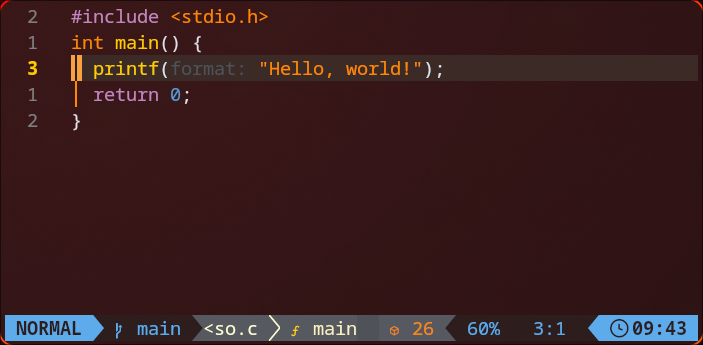
\includegraphics[width=\columnwidth]{media/t03/vimModoNormalInicio.png}
    \caption{Inicialización de sesión en Vim y estado por defecto en modo Normal \parencite[\S 2, p.\ 28]{oualline2001vim}.}
    \label{fig:vimModoNormalInicio}
\end{figure}

\subsection{Captura y modificación en modo Inserción}
\label{subsec:capturaModoInsercion}

Al pulsar la tecla \texttt{i}, el editor conmuta al modo Inserción, emitiendo secuencias ANSI para transformar el cursor en una línea vertical e indicando \texttt{-- INSERT --} en la barra de estado. En este estado se redacta un programa en C enfocado en llamadas al sistema para gestión de procesos (\texttt{fork()}, \texttt{getpid()} y \texttt{wait()}). Al concluir, la tecla \texttt{<Esc>} (o \texttt{Ctrl + [}) retorna al modo Normal, sincronizando páginas sucias con el archivo \texttt{.swp} en almacenamiento \parencite[\S 2, p.\ 32]{oualline2001vim}, como muestra la Img.~\ref{fig:vimModoInsercion}.

\begin{figure}[htbp]
    \centering
    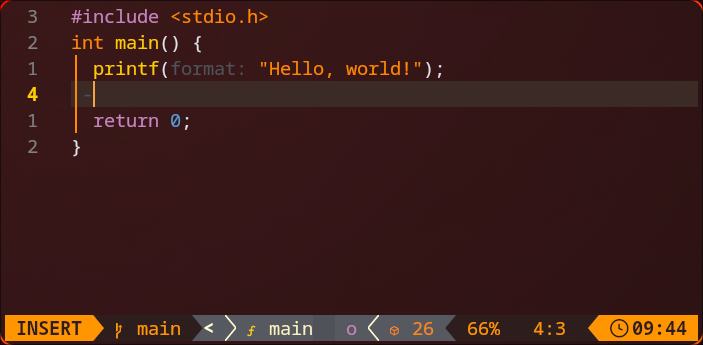
\includegraphics[width=\columnwidth]{media/t03/vimModoInsercion.png}
    \caption{Ingreso interactivo de código fuente en modo Inserción con indicador de estado \parencite[\S 2, p.\ 32]{oualline2001vim}.}
    \label{fig:vimModoInsercion}
\end{figure}

\subsection{Operaciones estructurales en modo Normal}
\label{subsec:operacionesEstructuralesModoNormal}

En modo Normal, las modificaciones se rigen por la gramática de la Ecuación~\eqref{eq:gramaticaVi}. La instrucción \texttt{yy} copia la línea del cursor al registro anónimo, y \texttt{p} la inserta en la posición inferior, mientras que \texttt{dd} suprime sentencias completas y \texttt{cw} sustituye palabras clave. El operador punto (\texttt{.}) reejecuta la última acción atómica, y el historial de cambios permite deshacer con \texttt{u} o rehacer con \texttt{Ctrl + r} \parencite[\S 2, p.\ 36]{oualline2001vim}. La Img.~\ref{fig:vimComandoOperador} documenta la duplicación y ajuste de variables del proceso.

\begin{figure}[htbp]
    \centering
    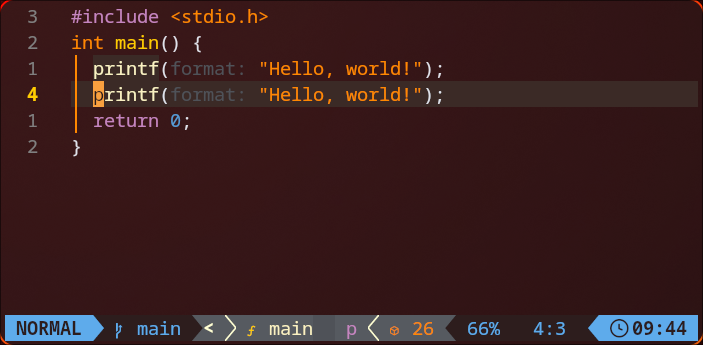
\includegraphics[width=\columnwidth]{media/t03/vimComandoOperador.png}
    \caption{Aplicación de operadores gramaticales y movimientos estructurales en modo Normal \parencite[\S 2, p.\ 36]{oualline2001vim}.}
    \label{fig:vimComandoOperador}
\end{figure}

\subsection{Selección por bloques en modo Visual}
\label{subsec:seleccionBloquesModoVisual}

El modo Visual provee selección estructurada en variantes por carácter (\texttt{v}), línea (\texttt{V}) o bloque matricial (\texttt{Ctrl + v}). Mediante el modo bloque visual, el operador delimita una columna rectangular vertical con las teclas \texttt{j} o \texttt{k} sobre múltiples líneas de código. Al pulsar \texttt{I}, redactar los caracteres de comentario (\texttt{// }) y presionar \texttt{<Esc>}, Vim propaga instantáneamente la modificación a todas las líneas del bloque seleccionado \parencite[\S 4, p.\ 85]{oualline2001vim}, como se aprecia en la Img.~\ref{fig:vimModoVisualBloque}.

\begin{figure}[htbp]
    \centering
    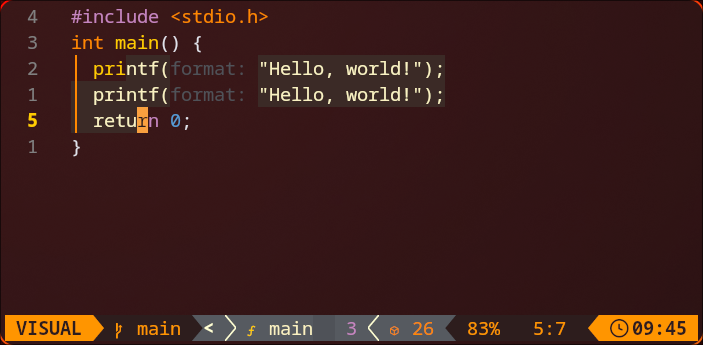
\includegraphics[width=\columnwidth]{media/t03/vimModoVisualBloque.png}
    \caption{Selección matricial de columnas en modo Visual Bloque para edición concurrente \parencite[\S 4, p.\ 85]{oualline2001vim}.}
    \label{fig:vimModoVisualBloque}
\end{figure}

\subsection{Comandos de sustitución y persistencia en modo Ex}
\label{subsec:comandosSustitucionPersistenciaModoEx}

El modo Ex se invoca con el carácter \texttt{:}. La directiva \texttt{:\%s/int/pid\_t/gc} analiza el búfer completo mediante expresiones regulares, solicitando confirmación interactiva (\texttt{c}) para sustituir el tipo primitivo por el identificador del kernel \texttt{pid\_t}. Finalmente, la instrucción \texttt{:wq} sincroniza el búfer con el inodo en disco mediante \texttt{write()} y \texttt{fsync()}, elimina el archivo \texttt{.swp} y restaura la terminal al modo canónico del sistema operativo \parencite{ieee2018posixvi}, tal como se expone en la Img.~\ref{fig:vimModoExGuardado}.

\begin{figure}[htbp]
    \centering
    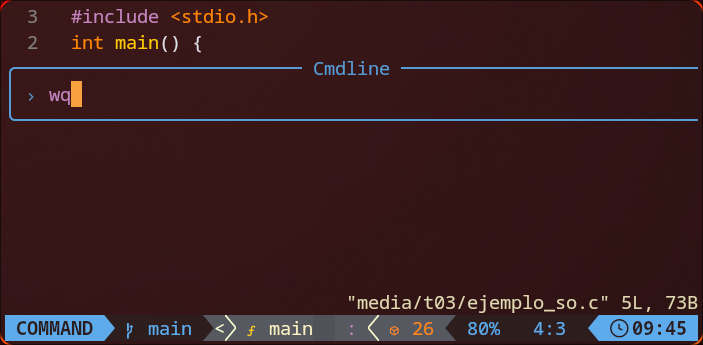
\includegraphics[width=\columnwidth]{media/t03/vimModoExGuardado.png}
    \caption{Ejecución de directivas globales en modo Ex y persistencia en disco con \texttt{:wq} \parencite{ieee2018posixvi}.}
    \label{fig:vimModoExGuardado}
\end{figure}

\section{Estructura de directorios: rutas absolutas y relativas}
\label{sec:estructuraDirectoriosRutas}

El sistema de archivos proporciona el mecanismo fundamental para la persistencia organizada, denominación y recuperación de la información en almacenamiento secundario. Para que el usuario y los procesos del sistema interactúen con los archivos sin requerir el direccionamiento físico por sectores o bloques, los sistemas operativos articulan una estructura jerárquica de directorios en forma de árbol invertido \parencite[\S 12.2, p.\ 535]{stallings2018operating}. Esta sección analiza la gestión del contexto de trabajo y formaliza la distinción operativa entre rutas absolutas y relativas en núcleos POSIX y Windows NT.

\subsection{Jerarquía del sistema de archivos y directorio de trabajo}
\label{subsec:jerarquiaDirectorioTrabajo}

En la arquitectura de sistemas tipo UNIX y GNU/Linux, el sistema de archivos virtual (\textit{virtual file system}, VFS) unifica todos los dispositivos de almacenamiento físico y sistemas lógicos en un único espacio de nombres jerárquico que desciende desde un nodo raíz global denominado \texttt{/} (\textit{root}). Por el contrario, Microsoft Windows NT estructura su espacio accesible mediante letras de unidad independientes asignadas a volúmenes lógicos (\texttt{C:\textbackslash}, \texttt{D:\textbackslash}), las cuales son gestionadas internamente por el Administrador de Objetos del núcleo como enlaces simbólicos hacia dispositivos nativos (como \texttt{\textbackslash Device\textbackslash HarddiskVolume1}) \parencite[\S 21.6, p.\ 1058]{deitel2004operating}.

Para resolver nombres de archivo de forma contextual, el sistema operativo vincula a cada proceso activo un atributo denominado directorio de trabajo actual (\textit{current working directory}, CWD). Esta propiedad reside en la estructura de control del proceso en memoria del núcleo: en Linux, dentro de la estructura \texttt{task\_struct->fs->pwd} (compuesta por punteros al inodo y a la entrada de directorio o \textit{dentry}), y en Windows, en los parámetros del proceso dentro del bloque de entorno del proceso (\textit{process environment block}, PEB). Cuando un proceso inicia su ejecución, hereda el CWD de su proceso padre (mediante \texttt{fork()} o \texttt{CreateProcess()}), pudiendo alterarlo dinámicamente durante su ciclo de vida mediante la llamada al sistema \texttt{chdir()} en POSIX o \texttt{SetCurrentDirectory()} en la API Win32 \parencite[\S 6.3, p.\ 309]{carretero2001sistemas}.

\subsection{Definición formal de ruta absoluta y ruta relativa}
\label{subsec:definicionRutasAbsolutaRelativa}

La localización de cualquier entidad dentro del árbol jerárquico se expresa mediante una trayectoria o ruta (\textit{pathname}), la cual consiste en una secuencia de identificadores textuales delimitados por separadores de directorio (\texttt{/} en UNIX y \texttt{\textbackslash} en Windows) \parencite[\S 10.3, p.\ 342]{silberschatz2006fundamentos}:

\begin{enumerate}[noitemsep, topsep=2pt]
    \item \textbf{Ruta absoluta (\textit{absolute path}):} Es una trayectoria canónica e invariable que especifica la ubicación de un archivo o directorio comenzando inequívocamente desde el nodo raíz del sistema de archivos (\texttt{/} en entornos POSIX o la letra de unidad seguida del delimitador de raíz \texttt{C:\textbackslash} en Windows). Su resolución es completamente autónoma e independiente del CWD del proceso emisor: dos procesos con directorios de trabajo dispares que invoquen una misma ruta absoluta (ej. \texttt{/etc/passwd} o \texttt{C:\textbackslash Windows\textbackslash System32\textbackslash drivers}) accederán idénticamente al mismo nodo físico en el almacenamiento secundario.
    \item \textbf{Ruta relativa (\textit{relative path}):} Es una trayectoria contextual que no inicia con el delimitador de raíz, estableciendo su origen de búsqueda a partir del CWD del proceso que la invoca. Su interpretación depende enteramente del estado dinámico del proceso: la referencia \texttt{config/datos.txt} se resuelve como \texttt{/home/usuario/config/datos.txt} si el CWD es \texttt{/home/usuario}, pero fallará o apuntará a otro inodo si el proceso migra su contexto a \texttt{/var/log}.
\end{enumerate}

Para posibilitar la navegación ascendente y la referencia local en rutas relativas, los sistemas de archivos incorporan de manera obligatoria en cada directorio dos entradas especiales: el punto (\texttt{.}), que constituye un enlace duro reflexivo hacia el propio directorio actual, y el doble punto (\texttt{..}), que apunta directamente al inodo del directorio padre en la jerarquía \parencite[\S 10.3, p.\ 343]{silberschatz2006fundamentos}. De este modo, expresiones como \texttt{../../bin/script.sh} ascienden dos niveles jerárquicos desde el CWD antes de descender al nodo objetivo.

\subsection{Mecanismos de resolución en núcleos POSIX y Windows NT}
\label{subsec:mecanismosResolucionNucleos}

En el espacio del núcleo, la conversión de una ruta textual en una referencia a inodo o manejador de archivo (\textit{handle}) exige un proceso iterativo de resolución componente por componente denominado recorrido de trayectoria (\textit{path walking}).

En sistemas GNU/Linux, el núcleo ejecuta la rutina interna \texttt{path\_walk()} del VFS. Si la ruta inicia con \texttt{/}, la resolución arranca desde el inodo raíz apuntado por \texttt{current->fs->root}; si no, inicia en \texttt{current->fs->pwd}. Para minimizar los costosos accesos de lectura a disco, el núcleo consulta la memoria caché de entradas de directorio (\textit{dentry cache} o \textit{dcache}), verificando secuencialmente los permisos de ejecución (\texttt{x}) necesarios para atravesar cada subdirectorio intermedio. En entornos modernos, las llamadas al sistema clásicas basadas en rutas globales (como \texttt{open()}) han sido complementadas por variantes relativas orientadas a descriptores de archivo, tales como \texttt{openat()} y \texttt{unlinkat()}. Estas funciones reciben un descriptor abierto de directorio (\textit{dirfd}) junto a una ruta relativa, permitiendo al proceso fijar atómicamente el contexto de resolución y mitigando condiciones de carrera de verificación frente a uso (\textit{time-of-check to time-of-use}, TOCTOU) en software multi-hilo \parencite{carretero2001sistemas}.

En Windows NT, las llamadas de la API Win32 (\texttt{CreateFile}) se canalizan hacia la llamada nativa \texttt{NtCreateFile}. El Administrador de Objetos del núcleo antepone el espacio de nombres de dispositivos de usuario (\texttt{\textbackslash ??\textbackslash C:\textbackslash...}), normaliza barras inclinadas y consulta las estructuras del sistema de archivos NTFS para resolver entradas de índice en la tabla maestra de archivos (\textit{master file table}, MFT) o procesar puntos de reanálisis (\textit{reparse points}) asociados a enlaces simbólicos y uniones de directorios.

La Tabla~\ref{tab:comparativaRutasSistemas} sintetiza las diferencias técnicas y de diseño entre rutas absolutas y relativas.

\begin{table}[htbp]
\centering
\footnotesize
\renewcommand{\arraystretch}{1.08}
\renewcommand{\tabularxcolumn}[1]{m{#1}}
\setlength{\emergencystretch}{1.5em}
\caption{Comparativa técnica y funcional entre rutas absolutas y relativas.}
\label{tab:comparativaRutasSistemas}
\begin{tabularx}{\textwidth}{>{\centering\arraybackslash}m{2.8cm} X X}
\toprule
\textbf{Criterio técnico} & \textbf{Ruta absoluta} & \textbf{Ruta relativa} \\
\midrule
\textbf{Origen sintáctico} & Inicia estrictamente en la raíz (\texttt{/} en UNIX; \texttt{<unidad>:\textbackslash} en Windows). & Inicia sin separador de raíz; referenciada al contexto actual (\texttt{./}, \texttt{../} o nombre directo). \\
\addlinespace
\textbf{Dependencia del CWD} & Invariante; no se altera ante modificaciones en el estado del proceso ejecutor. & Dependiente; la resolución final cambia si el proceso modifica su CWD con \texttt{chdir()}. \\
\addlinespace
\textbf{Resolución en el SO} & Recorrido jerárquico desde \texttt{fs->root} o volumen lógico asignado. & Recorrido a partir de \texttt{fs->pwd} o descriptor de directorio relativo (\texttt{dirfd} en \texttt{openat}). \\
\addlinespace
\textbf{Portabilidad} & Baja; acoplada a la disposición absoluta de directorios y volúmenes de un equipo específico. & Elevada; permite empaquetar árboles de proyectos y dependencias autocontenidas. \\
\addlinespace
\textbf{Seguridad de concurrencia} & Susceptible a sustitución encubierta de rutas en entornos multiusuario. & Permite acceso atómico mediante descriptores seguros (\texttt{openat()}) frente a TOCTOU. \\
\bottomrule
\end{tabularx}
\end{table}

\section{Comandos de terminal en sistemas GNU/Linux}
\label{sec:comandosTerminalLinux}

La interfaz de línea de comandos (\textit{command-line interface}, CLI) en sistemas operativos GNU/Linux constituye el entorno primordial para la administración del sistema, la automatización mediante guiones (\textit{shell scripts}) y el control de procesos. Lejos de ser un mero intermediario textual, el shell actúa como un potente lenguaje de programación interpretado que se comunica de forma directa con los servicios ejecutivos del núcleo mediante llamadas al sistema normalizadas por el estándar POSIX \parencite[\S 2.2, p.\ 48]{silberschatz2006fundamentos}. Esta sección analiza la arquitectura de ejecución de comandos y detalla diez de las utilidades de terminal más representativas del entorno.

\subsection{Arquitectura del shell y ejecución de utilidades}
\label{subsec:arquitecturaShellEjecucion}

El shell (predominantemente GNU Bash o Zsh en distribuciones contemporáneas) opera en espacio de usuario siguiendo un bucle clásico de lectura, evaluación, impresión y repetición (\textit{read-eval-print loop}, REPL). Al recibir una línea de comandos, el analizador léxico segmenta la cadena en componentes léxicos (\textit{tokens}), procesa expansiones de variables de entorno y comodines (\textit{globbing}), y clasifica la instrucción en una de dos categorías estructurales: comandos internos (\textit{built-ins}) y ejecutables externos \parencite[\S 2.4, p.\ 48]{carretero2001sistemas}.

Los comandos internos (como \texttt{cd}, \texttt{pwd} o \texttt{exit}) se ejecutan directamente dentro del espacio de memoria del propio proceso del shell. Esta integración es indispensable para órdenes que alteran el estado interno del proceso, como modificar el directorio de trabajo activo (CWD) o definir variables de entorno, ya que un proceso hijo aislado no puede mutar los descriptores ni la estructura \texttt{task\_struct} de su proceso padre. Por el contrario, los comandos externos corresponden a archivos binarios ubicados en directorios del sistema (como \texttt{/bin}, \texttt{/usr/bin} o \texttt{/usr/local/bin}), localizados a través de la variable de entorno \texttt{PATH}. Para ejecutarlos, el shell invoca la llamada al sistema \texttt{fork()} para clonar su hilo de ejecución y \texttt{execve()} para reemplazar la imagen del proceso hijo con el nuevo binario, coordinando la sincronización y el estado de salida mediante \texttt{waitpid()} \parencite[\S 3.2, p.\ 120]{stallings2018operating}.

Asimismo, el shell administra los tres descriptores de archivo estándar asignados por defecto a cada proceso: entrada estándar (\texttt{stdin}, descriptor 0), salida estándar (\texttt{stdout}, descriptor 1) y error estándar (\texttt{stderr}, descriptor 2). Mediante llamadas \texttt{dup2()} y \texttt{pipe()}, el shell posibilita la redirección de flujos hacia archivos en disco (\texttt{>}, \texttt{>>}, \texttt{<}) y la interconexión concurrente de comandos mediante tuberías (\textit{pipelines}, \texttt{|}), permitiendo canalizar la salida de un proceso directamente hacia la entrada del siguiente en memoria sin recurrir a almacenamiento secundario intermedio.

\subsection{Catálogo de diez comandos fundamentales}
\label{subsec:catalogoDiezComandosLinux}

Para interactuar eficazmente con el subsistema de archivos, la administración de memoria y el control de tareas en GNU/Linux, existe un conjunto de diez utilidades fundamentales cuya operatividad técnica se desglosa a continuación:

\begin{enumerate}[noitemsep, topsep=2pt]
    \item \textbf{\texttt{ls} (\textit{list}):} Enumera las entradas contenidas en un directorio. En el núcleo, invoca la llamada al sistema \texttt{getdents64()} para leer bloques de entradas de directorio y consulta metadatos de inodos con \texttt{statx()} (o \texttt{lstat()} para enlaces simbólicos). Opciones como \texttt{-l} generan el listado largo (permisos POSIX, propietario, grupo, tamaño y marca temporal), \texttt{-a} expone archivos ocultos (cuyo nombre inicia con punto) y \texttt{-h} humaniza el tamaño en potencias de 1024.
    \item \textbf{\texttt{cd} (\textit{change directory}):} Modifica el directorio de trabajo del proceso del shell. Al ser un comando interno, invoca directamente la llamada \texttt{chdir()}, actualizando el puntero \texttt{fs->pwd} en la estructura del kernel. La invocación sin argumentos o con \texttt{\textasciitilde} traslada al directorio de inicio del usuario (\texttt{\$HOME}), mientras que \texttt{cd -} retorna al directorio previo (\texttt{\$OLDPWD}).
    \item \textbf{\texttt{pwd} (\textit{print working directory}):} Imprime la ruta absoluta del CWD activo. Invoca la llamada al sistema \texttt{getcwd()}, la cual inspecciona la tabla de dentries en el VFS para reconstruir la cadena canónica desde la raíz hasta el nodo actual. La bandera \texttt{-P} resuelve enlaces simbólicos mostrando la ruta física real.
    \item \textbf{\texttt{mkdir} (\textit{make directory}):} Crea nuevos nodos de tipo directorio en el sistema de archivos. Ejecuta la llamada al sistema \texttt{mkdir()} o \texttt{mkdirat()}, asignando un nuevo inodo con los bits de directorio habilitados y aplicando la máscara de modo de creación de archivos (\texttt{umask}). Con la opción \texttt{-p} (\textit{parents}), crea recursivamente toda la jerarquía de subdirectorios faltantes sin arrojar errores si ya existen.
    \item \textbf{\texttt{cp} (\textit{copy}):} Duplica archivos o árboles de directorios. En núcleos Linux contemporáneos, utiliza llamadas optimizadas como \texttt{copy\_file\_range()} o \texttt{sendfile()}, permitiendo clonaciones directas entre descriptores en el kernel o reflejos instantáneos a nivel de bloques en sistemas de archivos con copia en escritura (\textit{copy-on-write}, CoW) como Btrfs. La bandera \texttt{-r} aplica copia recursiva y \texttt{-p} preserva marcas temporales y permisos originales.
    \item \textbf{\texttt{mv} (\textit{move}):} Reubica o renombra nodos en la jerarquía. Si el destino reside en el mismo sistema de archivos, ejecuta la llamada atómica \texttt{rename()} o \texttt{renameat2()}, actualizando las entradas de directorio en disco sin copiar datos físicos. Si involucra diferentes dispositivos montados, recurre a una copia profunda seguida de la supresión del origen.
    \item \textbf{\texttt{rm} (\textit{remove}):} Elimina enlaces de archivos y directorios. En archivos regulares ejecuta \texttt{unlink()}, decrementando el contador de enlaces duros (\textit{hard links}) del inodo; cuando este llega a cero y ningún proceso retiene descriptores abiertos sobre él, el núcleo libera los bloques de datos asociados en disco. La opción \texttt{-r} efectúa borrado recursivo en árboles de directorios y \texttt{-f} fuerza la operación suprimiendo solicitudes de confirmación.
    \item \textbf{\texttt{cat} (\textit{concatenate}):} Lee flujos secuenciales de datos desde archivos o \texttt{stdin} y los vuelca hacia \texttt{stdout}. Implementa bucles de lectura y escritura en memoria mediante \texttt{read()} y \texttt{write()}, resultando idóneo para inspeccionar archivos de configuración cortos o concatenar segmentos de texto mediante tuberías. Opciones como \texttt{-n} numeran las líneas emitidas.
    \item \textbf{\texttt{grep} (\textit{global regular expression print}):} Analiza flujos de texto en busca de patrones que coincidan con una expresión regular. Utiliza algoritmos de concordancia de patrones (como Boyer-Moore y autómatas finitos deterministas) procesando búferes intermedios con mínima latencia. Banderas como \texttt{-i} ignoran mayúsculas y minúsculas, \texttt{-r} realiza búsqueda recursiva en árboles y \texttt{-v} invierte el criterio filtrando líneas no coincidentes.
    \item \textbf{\texttt{ps} (\textit{process status}):} Reporta una instantánea de los procesos activos en ejecución. En GNU/Linux, no realiza sondeos destructivos; en su lugar, examina el sistema de archivos virtual \texttt{/proc}, donde el núcleo expone estructuras dinámicas de cada PID (\texttt{/proc/[pid]/stat}, \texttt{status}, \texttt{cmdline}). La sintaxis clásica \texttt{ps aux} o la normalizada POSIX \texttt{ps -ef} detallan el usuario emisor, consumo de CPU y memoria, estado de planificación y comando de invocación.
\end{enumerate}

La Tabla~\ref{tab:catalogoComandosLinux} resume las características sintácticas, parámetros esenciales y llamadas al sistema asociadas a este catálogo de comandos.

\begin{table}[htbp]
\centering
\footnotesize
\renewcommand{\arraystretch}{1.08}
\renewcommand{\tabularxcolumn}[1]{m{#1}}
\setlength{\emergencystretch}{1.5em}
\caption{Catálogo técnico de diez comandos fundamentales en GNU/Linux.}
\label{tab:catalogoComandosLinux}
\begin{tabularx}{\textwidth}{>{\centering\arraybackslash}m{2.0cm} >{\centering\arraybackslash}m{2.4cm} >{\centering\arraybackslash}m{2.4cm} X}
\toprule
\textbf{Comando} & \textbf{Sintaxis representativa} & \textbf{Llamada al sistema} & \textbf{Función y semántica en el sistema operativo} \\
\midrule
\texttt{ls} & \texttt{ls -lah} & \texttt{getdents64}, \texttt{statx} & Lista contenidos de directorio recuperando metadatos y permisos desde inodos. \\
\addlinespace
\texttt{cd} & \texttt{cd /var/log} & \texttt{chdir} (\textit{builtin}) & Modifica el directorio de trabajo (CWD) del proceso en \texttt{task\_struct->fs->pwd}. \\
\addlinespace
\texttt{pwd} & \texttt{pwd -P} & \texttt{getcwd} & Reconstruye e imprime la ruta canónica absoluta hacia el CWD del proceso. \\
\addlinespace
\texttt{mkdir} & \texttt{mkdir -p ruta/dir} & \texttt{mkdir}, \texttt{mkdirat} & Asigna un inodo de directorio y crea las entradas correspondientes en disco. \\
\addlinespace
\texttt{cp} & \texttt{cp -rp orig dest} & \texttt{copy\_file\_range} & Duplica archivos o árboles preservando metadatos; optimizado en el kernel. \\
\addlinespace
\texttt{mv} & \texttt{mv arch nuevo} & \texttt{rename}, \texttt{renameat2} & Reubica o renombra nodos atómicamente alterando enlaces de directorio. \\
\addlinespace
\texttt{rm} & \texttt{rm -rf temp/} & \texttt{unlink}, \texttt{rmdir} & Decrementa enlaces duros del inodo y libera bloques de datos en almacenamiento. \\
\addlinespace
\texttt{cat} & \texttt{cat -n arch.txt} & \texttt{read}, \texttt{write} & Vuelca secuencialmente flujos de bytes hacia el descriptor \texttt{stdout}. \\
\addlinespace
\texttt{grep} & \texttt{grep -ri \textquotedbl patrón\textquotedbl} & Búferes VFS / regex & Filtra líneas por concordancia de expresiones regulares mediante autómatas. \\
\addlinespace
\texttt{ps} & \texttt{ps aux} / \texttt{ps -ef} & Lectura en \texttt{/proc} & Inspecciona estructuras de procesos y estados de hilos expuestos por el kernel. \\
\bottomrule
\end{tabularx}
\end{table}

\section{Comandos del intérprete CMD en Windows}
\label{sec:comandosCmdWindows}

En el sistema operativo Microsoft Windows, el símbolo del sistema o intérprete de comandos (\texttt{cmd.exe}) representa el procesador de órdenes tradicional para la automatización administrativa mediante archivos por lotes (\textit{batch files}, \texttt{.bat} y \texttt{.cmd}) y el control directo del sistema operativo. Aunque Windows incorpora entornos contemporáneos más complejos como PowerShell, \texttt{cmd.exe} permanece como un componente medular del subsistema Win32, caracterizado por una latencia de inicialización mínima, compatibilidad estricta con utilidades heredadas y acceso directo a las interfaces ejecutivas del núcleo Windows NT \parencite[\S 21.4, p.\ 1045]{deitel2004operating}.

\subsection{Arquitectura de cmd.exe y llamadas al sistema}
\label{subsec:arquitecturaCmdEjecucion}

A diferencia del shell de UNIX, que interactúa directamente con el controlador de pseudoterminal del núcleo, \texttt{cmd.exe} opera como un proceso Win32 desacoplado de la ventana física de visualización. Históricamente, la consola gráfica era gestionada por el proceso del subsistema cliente/servidor (\texttt{csrss.exe}); a partir de Windows 7, esta responsabilidad se transfirió al proceso de alojamiento de ventanas de consola (\textit{Console Window Host}, \texttt{conhost.exe}) para mitigar vulnerabilidades de seguridad, y más recientemente a la infraestructura de pseudoconsolas (\textit{ConPTY}) integrada en Windows Terminal.

Al procesar una línea de comandos, el analizador sintáctico de \texttt{cmd.exe} discrimina entre dos categorías de instrucciones: comandos internos y comandos externos. Los comandos internos se encuentran compilados directamente dentro del código ejecutable de \texttt{cmd.exe} (como \texttt{DIR}, \texttt{CD}, \texttt{MD}, \texttt{COPY}, \texttt{DEL} o \texttt{TYPE}). Su ejecución ocurre en el contexto del propio hilo del intérprete, lo cual es imprescindible para funciones que alteran el entorno del proceso (como modificar el CWD en el bloque PEB mediante \texttt{SetCurrentDirectoryW} o actualizar variables de entorno en la memoria local). Por su parte, los comandos externos corresponden a archivos ejecutables independientes (con extensiones \texttt{.exe}, \texttt{.com}) ubicados habitualmente en el directorio del sistema (\texttt{C:\textbackslash Windows\textbackslash System32}).

Para ejecutar una utilidad externa (como \texttt{tasklist.exe} o \texttt{robocopy.exe}), \texttt{cmd.exe} invoca la función de la API Win32 \texttt{CreateProcessW()}, la cual transfiere la solicitud a la llamada al sistema nativa del núcleo \texttt{NtCreateUserProcess()} (o \texttt{NtCreateProcessEx()}) \parencite[\S 2.3, p.\ 52]{silberschatz2006fundamentos}. Esta llamada crea el objeto de proceso y su hilo inicial, asigna el espacio de direcciones virtuales, enlaza los manejadores de entrada y salida estándar (\texttt{STD\_INPUT\_HANDLE}, \texttt{STD\_OUTPUT\_HANDLE}, \texttt{STD\_ERROR\_HANDLE}) y entrega los argumentos a través de la línea de comandos en el bloque PEB \parencite[\S 3.2, p.\ 125]{stallings2018operating}.

\subsection{Catálogo de diez comandos fundamentales}
\label{subsec:catalogoDiezComandosWindows}

A continuación se analizan diez de los comandos más utilizados en \texttt{cmd.exe} en Windows 10 y Windows 11 para la administración de archivos, diagnóstico del almacenamiento y supervisión de procesos:

\begin{enumerate}[noitemsep, topsep=2pt]
    \item \textbf{\texttt{dir} (\textit{directory}):} Lista los archivos y subdirectorios presentes en la ruta especificada. A nivel del núcleo, utiliza las funciones de la API Win32 \texttt{FindFirstFileW()} y \texttt{FindNextFileW()}, consultando los registros de índice de la tabla maestra de archivos (MFT) en particiones NTFS. Opciones como \texttt{/A} filtran por atributos específicos (archivos ocultos o de sistema), \texttt{/S} realiza una búsqueda recursiva a través de todos los subdirectorios y \texttt{/Q} expone la identidad del propietario del archivo.
    \item \textbf{\texttt{cd} / \texttt{chdir} (\textit{change directory}):} Muestra o modifica el directorio de trabajo del proceso. Al ser un comando interno, interactúa con la estructura PEB del intérprete invocando \texttt{SetCurrentDirectoryW()}. La inclusión del modificador \texttt{/D} resulta indispensable cuando la conmutación de contexto involucra cambiar simultáneamente de letra de unidad lógica (por ejemplo, conmutar de \texttt{C:\textbackslash} a \texttt{D:\textbackslash Proyectos}).
    \item \textbf{\texttt{md} / \texttt{mkdir} (\textit{make directory}):} Crea nuevos directorios en el sistema de archivos mediante la API \texttt{CreateDirectoryW()}. En las implementaciones modernas de \texttt{cmd.exe}, este comando incorpora una capacidad avanzada: si se le proporciona una ruta compuesta que contiene subdirectorios intermedios inexistentes (ej. \texttt{md config\textbackslash logs\textbackslash 2026}), crea de forma atómica y transparente todos los niveles del árbol sin requerir parámetros adicionales.
    \item \textbf{\texttt{copy}:} Duplica uno o varios archivos hacia otra ubicación de almacenamiento invocando \texttt{CopyFileW()} o manejando flujos de datos con \texttt{ReadFile()} y \texttt{WriteFile()}. Presenta la facultad técnica de concatenar múltiples archivos de texto plano o binarios en un único destino mediante el operador de adición (ej. \texttt{copy arch1.txt + arch2.txt destino.txt}), y permite verificar la integridad de la escritura mediante el parámetro \texttt{/V}.
    \item \textbf{\texttt{move}:} Reubica archivos o renombra directorios completos en el árbol jerárquico. Si el origen y el destino residen dentro del mismo volumen lógico, ejecuta la función \texttt{MoveFileExW()} con la bandera \texttt{MOVEFILE\_COPY\_ALLOWED}, actualizando los punteros de nodo en la MFT sin duplicar los bloques de datos físicos. Si involucra volúmenes distintos, realiza una copia profunda seguida de la eliminación del archivo original.
    \item \textbf{\texttt{del} / \texttt{erase}:} Suprime uno o varios archivos del almacenamiento secundario mediante \texttt{DeleteFileW()}, marcando los clústeres correspondientes como espacio disponible en el mapa de bits del sistema de archivos. Parámetros como \texttt{/F} fuerzan la eliminación de archivos con atributo de solo lectura, \texttt{/S} propaga la supresión recursivamente en subcarpetas y \texttt{/Q} activa el modo silencioso suprimiendo solicitudes interactivas de confirmación.
    \item \textbf{\texttt{type}:} Despliega en la consola el contenido bruto de archivos de texto sin paginación (análogo funcional de \texttt{cat} en UNIX). Lee secuencialmente el archivo mediante \texttt{ReadFile()} y vuelca los bytes hacia el manejador de salida de la consola a través de \texttt{WriteConsoleW()} o \texttt{WriteFile()}, permitiendo redirigir su flujo hacia filtros mediante tuberías.
    \item \textbf{\texttt{tasklist}:} Utilidad externa (\texttt{tasklist.exe}) que reporta el inventario completo de tareas y procesos activos. Consulta las estructuras del núcleo mediante la interfaz Toolhelp32 o llamadas nativas a \texttt{NtQuerySystemInformation()}, exponiendo el nombre de imagen, identificador de proceso (PID), nombre de sesión, número de sesión y el consumo de memoria en el conjunto de trabajo (\textit{working set}). La opción \texttt{/SVC} detalla los servicios de Windows alojados en cada instancia de \texttt{svchost.exe}, y \texttt{/FI} aplica filtros avanzados de consulta.
    \item \textbf{\texttt{taskkill}:} Herramienta externa (\texttt{taskkill.exe}) diseñada para finalizar procesos en ejecución. Localiza el proceso mediante \texttt{OpenProcess()} solicitando el privilegio de seguridad \texttt{PROCESS\_TERMINATE} e invoca la llamada al sistema \texttt{TerminateProcess()}. Banderas esenciales incluyen \texttt{/PID <id>} o \texttt{/IM <imagen.exe>}, \texttt{/F} para imponer una terminación forzada no negociable y \texttt{/T} para finalizar recursivamente el proceso objetivo y todo su árbol de procesos secundarios subordinados.
    \item \textbf{\texttt{robocopy} (\textit{robust file copy}):} Utilidad avanzada de replicación y sincronización de estructuras de directorios (\texttt{robocopy.exe}). Diseñada para entornos empresariales tolerantes a fallos de red, soporta la reanudación automática de transferencias interrumpidas. Banderas críticas son \texttt{/E} (copia recursiva de subdirectorios, incluidos los vacíos), \texttt{/MIR} (modo espejo reflejo que sincroniza y purga destinos), \texttt{/SEC} (preserva listas de control de acceso NTFS / ACL y marcas de tiempo) y \texttt{/MT} (transferencia multi-hilo concurrente).
\end{enumerate}

La Tabla~\ref{tab:catalogoComandosWindows} sintetiza las propiedades técnicas, tipo de implementación y funciones asociadas a este catálogo de comandos en Windows.

\begin{table}[htbp]
\centering
\footnotesize
\renewcommand{\arraystretch}{1.08}
\renewcommand{\tabularxcolumn}[1]{m{#1}}
\setlength{\emergencystretch}{1.5em}
\caption{Catálogo técnico de diez comandos fundamentales en CMD de Windows.}
\label{tab:catalogoComandosWindows}
\begin{tabularx}{\textwidth}{>{\centering\arraybackslash}m{2.0cm} >{\centering\arraybackslash}m{2.4cm} >{\centering\arraybackslash}m{2.4cm} X}
\toprule
\textbf{Comando} & \textbf{Sintaxis representativa} & \textbf{Tipo y API Win32} & \textbf{Función y semántica en el sistema operativo} \\
\midrule
\texttt{dir} & \texttt{dir /A /S /Q} & Interno / \texttt{FindNextFileW} & Lista contenidos de directorio inspeccionando la MFT en particiones NTFS. \\
\addlinespace
\texttt{cd} & \texttt{cd /D D:\textbackslash datos} & Interno / \texttt{SetCurrentDirectory} & Modifica el CWD en el bloque PEB, conmutando opcionalmente de letra de unidad. \\
\addlinespace
\texttt{md} & \texttt{md ruta\textbackslash sub\textbackslash dir} & Interno / \texttt{CreateDirectoryW} & Crea carpetas físicas en disco, autogenerando niveles intermedios de jerarquía. \\
\addlinespace
\texttt{copy} & \texttt{copy a.txt+b.txt c.txt} & Interno / \texttt{CopyFileW} & Duplica y permite concatenar archivos con verificación de integridad opcional. \\
\addlinespace
\texttt{move} & \texttt{move orig dest} & Interno / \texttt{MoveFileExW} & Reubica o renombra nodos actualizando metadatos de directorio en la MFT. \\
\addlinespace
\texttt{del} & \texttt{del /F /S /Q arch} & Interno / \texttt{DeleteFileW} & Marca sectores como libres y desvincula el nodo del sistema de archivos. \\
\addlinespace
\texttt{type} & \texttt{type config.ini} & Interno / \texttt{WriteConsoleW} & Vuelca secuencialmente flujos de texto sin formato hacia el búfer de consola. \\
\addlinespace
\texttt{tasklist} & \texttt{tasklist /SVC /FI ...} & Externo / \texttt{Toolhelp32} & Monitorea procesos activos, servicios asociados y consumo de Working Set. \\
\addlinespace
\texttt{taskkill} & \texttt{taskkill /F /T /PID 12} & Externo / \texttt{TerminateProcess} & Envía señal de terminación forzada y recursiva a procesos y sus hilos hijos. \\
\addlinespace
\texttt{robocopy} & \texttt{robocopy orig dest /MIR} & Externo / E/S multi-hilo & Replicación robusta de árboles jerárquicos con preservación de ACL y reanudación. \\
\bottomrule
\end{tabularx}
\end{table}

\section{Análisis comparativo de interfaces y direccionamiento}
\label{sec:analisisComparativoInterfaces}

La divergencia evolutiva entre la familia de sistemas operativos POSIX y la arquitectura Windows NT ha forjado paradigmas marcadamente contrastantes en la interacción usuario-núcleo y la estructuración de recursos. Aunque ambas plataformas proveen entornos multitarea y multiusuario, sus premisas discrepan en el tratamiento de flujos de datos, la instanciación de procesos y la semántica de direccionamiento en almacenamiento secundario \parencite[\S 2.3, p.\ 51]{silberschatz2006fundamentos}.

\subsection{Comparativa entre entornos de línea de comandos}
\label{subsec:comparativaEntornosLineasComandos}

El modelo del shell en GNU/Linux concibe los componentes como archivos y privilegia flujos continuos de bytes en texto plano sin formato (\textit{unformatted text streams}) comunicados mediante tuberías unidireccionales (\texttt{|}) \parencite[\S 1.4, p.\ 38]{stallings2018operating}. En contraparte, \texttt{cmd.exe} en Windows NT opera como un invocador de funciones del subsistema Win32, interactuando mediante búferes de consola orientados a celdas administrados por ConPTY / \texttt{conhost.exe}. En el ciclo de vida de procesos, Linux adopta la bifurcación asíncrona con copia en escritura (\texttt{fork()}) y carga con \texttt{execve()} \parencite[\S 3.2, p.\ 122]{carretero2001sistemas}, permitiendo aislar y reconfigurar descriptores antes de ejecutar el binario; por el contrario, Windows NT implementa la creación ejecutiva monolítica y atómica mediante \texttt{NtCreateUserProcess()} (encapsulada en \texttt{CreateProcessW()}), asignando espacio virtual, mapeando el ejecutable PE y enlazando manejadores en una única llamada de alta complejidad \parencite[\S 21.4, p.\ 1044]{deitel2004operating}.

\subsection{Diferencias operativas en la gestión de rutas}
\label{subsec:diferenciasGestionRutas}

En el sistema de archivos, GNU/Linux articula un árbol unificado en el VFS desde una raíz canónica (\texttt{/}), integrando particiones y sistemas sintéticos (\texttt{/proc}, \texttt{/sys}) mediante puntos de montaje transparentes \parencite[\S 13.2, p.\ 455]{silberschatz2006fundamentos}. Por el contrario, Windows NT particiona el espacio en letras de unidad (\texttt{C:\textbackslash}, \texttt{D:\textbackslash}) mapeadas en \texttt{\textbackslash DosDevices}, manteniendo en el bloque PEB un CWD independiente por volumen. Asimismo, el VFS en POSIX es estrictamente sensible a mayúsculas (\textit{case-sensitive}), usa la barra ordinaria (\texttt{/}) y mitiga condiciones de carrera mediante descriptores relativos (\texttt{openat()}), mientras que el subsistema Win32 es insensible a mayúsculas (\textit{case-insensitive}), emplea la barra invertida (\texttt{\textbackslash}) y valida derechos de acceso evaluando listas DACL de forma centralizada al despachar \texttt{NtCreateFile()}.

La Tabla~\ref{tab:matrizComparativaEntornos} resume las diferencias estructurales y operativas entre los entornos POSIX / GNU/Linux y la arquitectura Windows NT.

\begin{table}[htbp]
\centering
\footnotesize
\renewcommand{\arraystretch}{1.08}
\renewcommand{\tabularxcolumn}[1]{m{#1}}
\setlength{\emergencystretch}{1.5em}
\caption{Matriz comparativa multidimensional entre entornos POSIX y Windows NT.}
\label{tab:matrizComparativaEntornos}
\begin{tabularx}{\textwidth}{>{\centering\arraybackslash}m{2.6cm} X X}
\toprule
\textbf{Criterio de diseño} & \textbf{Paradigma POSIX / GNU/Linux} & \textbf{Paradigma Windows NT (CMD / Win32)} \\
\midrule
\textbf{Filosofía de comunicación} & Flujos de bytes continuos en texto plano sin estructura (\texttt{stdout}, tuberías anónimas). & Mensajes de eventos, búferes de pantalla de consola (\texttt{conhost.exe}) y API Win32. \\
\addlinespace
\textbf{Modelo de procesos} & Bifurcación desacoplada \texttt{fork()} con copia en escritura (\textit{COW}) y carga con \texttt{execve()}. & Creación monolítica atómica mediante \texttt{CreateProcessW()} / \texttt{NtCreateUserProcess()}. \\
\addlinespace
\textbf{Jerarquía de directorios} & Árbol único unificado bajo la raíz canónica \texttt{/} mediante puntos de montaje del VFS. & Espacio de nombres particionado en letras de unidad (\texttt{C:\textbackslash}, \texttt{D:\textbackslash}) mapeadas en \texttt{\textbackslash DosDevices}. \\
\addlinespace
\textbf{Sintaxis y sensibilidad} & Sensible a mayúsculas (\textit{case-sensitive}); delimitador canónico de niveles \texttt{/}. & Insensible a mayúsculas (\textit{case-insensitive}); delimitador \texttt{\textbackslash} y caracteres reservados. \\
\addlinespace
\textbf{Gestión del CWD} & Puntero único a estructura \texttt{struct path} en el descriptor de proceso (\texttt{task\_struct}). & Múltiples CWD por unidad lógica persistidos en el bloque PEB del proceso. \\
\addlinespace
\textbf{Resolución y seguridad} & Resolución iterativa por inodos; mitigación TOCTOU vía descriptores relativos (\texttt{openat}). & Resolución MFT y comprobación centralizada de listas DACL/SACL mediante \texttt{NtCreateFile}. \\
\bottomrule
\end{tabularx}
\end{table}

\section{Conclusiones personales}
\label{sec:conclusionesPersonales}

El análisis sistemático de la interacción entre el usuario y el sistema operativo desarrollado en este trabajo pone de manifiesto que las interfaces contemporáneas, lejos de ser meras capas superficiales de presentación visual o interpretación sintáctica, constituyen extensiones directas de la arquitectura interna del núcleo. La gestión de atajos de teclado ilustra con notable claridad la intrincada colaboración asíncrona entre el silicio y el espacio de usuario: desde la generación de códigos de escaneo binarios en el controlador físico y el despacho de interrupciones de hardware hacia las rutinas ISR del procesador, hasta la normalización de códigos virtuales en mitades inferiores del kernel y su posterior enrutamiento por parte del compositor gráfico o el subsistema de ventanas. Este flujo evidencia cómo las decisiones de diseño a bajo nivel determinan de manera tajante la seguridad y la latencia del sistema; la transición desde la arquitectura histórica de X11 hacia compositores Wayland y portales de escritorio XDG fundamentados en aislamiento de memoria y paso de mensajes mediante D-Bus erradica vectores de intercepción pasiva (\textit{keylogging}) que durante décadas comprometieron la integridad del escritorio en entornos UNIX, equilibrando la inmediatez operativa con el confinamiento de privilegios.

En el ámbito de la edición interactiva de código y configuración de infraestructura, el estudio profundo del editor Vi y su evolución hacia Vim revela la vigencia y superioridad ergonómica del paradigma modal frente al modelo de inserción continua dominante en procesadores de texto y entornos integrados modernos. Concebir el editor como una máquina de estados finitos determinista sustentada en una gramática formal rigurosa transforma la edición en un lenguaje algebraico donde los operadores léxicos interactúan armónicamente con objetos de texto y cuantificadores numéricos. Al confinar los desplazamientos y comandos a la fila central del teclado alfanumérico, el modelo modal suprime drásticamente la sobrecarga biomecánica provocada por la conmutación constante hacia el ratón o el uso forzado de teclas modificadoras periféricas, reduciendo la fricción cognitiva en sesiones prolongadas de programación y administración remota. Asimismo, el desacoplamiento entre el búfer dinámico en memoria RAM y el archivo de intercambio temporal en disco ejemplifica una implementación magistral de tolerancia a fallos y concurrencia mediante cerrojos a nivel de proceso, garantizando la consistencia transaccional del código incluso ante anomalías intempestivas del entorno de ejecución.

La exploración comparativa de las interfaces de línea de comandos en GNU/Linux y Microsoft Windows permite dimensionar dos filosofías arquitectónicas divergentes pero altamente refinadas para el control de recursos. En el ecosistema POSIX, el principio fundamental de estructurar la comunicación mediante flujos unidireccionales de bytes en texto plano sin formato, concatenados mediante tuberías y primitivas estándar de entrada y salida, propicia la modularidad y la composición ortogonal de herramientas especializadas. Este enfoque, complementado por la bifurcación asíncrona de procesos mediante \texttt{fork()} bajo el esquema de copia en escritura y la posterior carga con \texttt{execve()}, otorga una flexibilidad granular insuperable para la automatización de tareas complejas en el centro de datos. En contraste, el intérprete \texttt{cmd.exe} y el subsistema Win32 abordan la interacción a través de búferes de pantalla de consola administrados por procesos anfitriones y la invocación atómica de funciones ejecutivas monolíticas en el núcleo Windows NT. Si bien este modelo demanda estructuras de datos más rígidas y una sobrecarga superior en la inicialización de procesos mediante \texttt{NtCreateUserProcess()}, ofrece una integración estrecha y determinista con el modelo de objetos, los descriptores de seguridad y las listas de control de acceso propias de la infraestructura corporativa de Microsoft.

Finalmente, la formalización técnica del direccionamiento jerárquico subraya el papel preponderante del sistema de archivos como organizador del estado persistente de la máquina. La confrontación entre el árbol unificado bajo la raíz canónica del VFS en GNU/Linux y el particionamiento en letras de unidad independientes en Windows NT refleja visiones ontológicas distintas sobre la abstracción del hardware. Mientras el VFS integra discos y recursos sintéticos bajo descriptores seguros (\texttt{openat()}) para evitar condiciones de carrera temporales, Windows mantiene contextos de trabajo independientes por volumen en el bloque PEB y valida los accesos mediante tablas MFT y el Gestor de Objetos. Dominar la distinción entre rutas absolutas invariantes y relativas contextuales constituye una competencia crítica de ingeniería para diseñar software portable, robusto y protegido contra ataques de secuestro de rutas.

\nocite{*}
\renewcommand*{\bibfont}{\small}
\setlength{\bibitemsep}{0.2\parsep}
\printbibliography[heading=bibintoc, title={Referencias}]

\end{document}
